\documentclass[a4paper,12pt]{article}

\usepackage{amsfonts, amsmath, amssymb, amsthm, dsfont, enumitem, fancyhdr, graphicx}
\usepackage[margin=0.9in, includehead, includefoot, heightrounded]{geometry}
\allowdisplaybreaks
\pagestyle{fancy}
\rhead{Erick Lin}

\newcommand{\norm}[1]{\left\lVert#1\right\rVert}
\newcommand*\dist{\mathop{\!\mathrm{d}}}
\DeclareMathOperator{\im}{Im}
\let\ker\relax %RedeclareMathOperator
\DeclareMathOperator{\ker}{Ker}
\renewcommand{\thesubsection}{\arabic{subsection}}
\newcommand*\sq{\mathbin{\vcenter{\hbox{\rule{.3ex}{.3ex}}}}}
\newcommand{\iso}{\approx}
\newtheorem{theorem}{Theorem}
\newtheorem{lemma}[theorem]{Lemma}

\begin{document}

\section*{MATH 6441 -- HW5 Solutions}
\subsection*{Section 2.1}
\begin{enumerate}
    \item[5.]
        \boldmath\textbf{Compute the simplicial homology groups of the Klein bottle $K$ using the $\Delta$-complex structure given below.
        }\unboldmath \par
        {\centering
            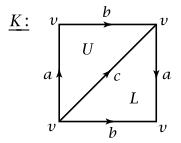
\includegraphics[scale=1]{klein_delta}
        \\}
        The $\Delta$-complex structure has one vertex $v$, three edges $a, b$, and $c$, and two $2$-simplices $U$ and $L$. $\partial_1 = 0$ since $\partial a = \partial b = \partial c = v - v = 0$, so $H_0^\Delta(K) = \ker\partial_0 = \Delta_0(K) \approx \mathbb{Z}$. $\partial_2 U = a + b - c$ and $\partial_2 L = a - b + c$, and $\{ a, b, a + b - c \}$ is a basis for $\ker\partial_1 = \Delta_1(K)$; it follows that taking the quotient $\ker\partial_1 / \im\partial_2 = H_1^\Delta(K)$ induces the relations $a + b - c = 0$ and $a - b + c = -2b = 0$, and thus we have $H_1^\Delta(K) \approx \mathbb{Z} \oplus \mathbb{Z}_2$ with basis the homology classes $[a]$ and $[b]$. Since there are no 3-simplices, $H_2^\Delta(K)$ is equal to $\ker\partial_2$, which is zero since $a + b - c$ and $a - b + c$ are linearly independent, meaning that $\partial(pU + qL) = p(a + b - c) + q(a - b + c) = 0$ only if $p = q = 0$. In conclusion, the simplicial homology groups are given by
        \begin{align*}
            H_n^\Delta(K) \approx \begin{cases}
                \mathbb{Z} &\text{for } n = 0 \\
                \mathbb{Z} \oplus \mathbb{Z}_2 &\text{for } n = 1 \\
                0 &\text{for } n \geq 2
            \end{cases}.
        \end{align*}

    \item[8.]
        \boldmath\textbf{Construct a 3-dimensional $\Delta$-complex $X$ from $n$ tetrahedra $T_1, \cdots, T_n$ by the following two steps. First arrange the tetrahedra in a cyclic pattern as in the figure, so that each $T_i$ shares a common vertical face with its two neighbors $T_{i - 1}$ and $T_{i + 1}$, subscripts being taken mod $n$. Then identify the bottom face of $T_i$ with the top face of $T_{i + 1}$ for each $i$. Show that the simplicial homology groups of $X$ in dimensions 0, 1, 2, 3 are $\mathbb{Z}$, $\mathbb{Z}_n$, $0$, $\mathbb{Z}$, respectively.
        }\unboldmath \par
        {\centering
            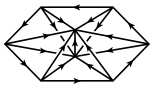
\includegraphics[scale=1]{hw5_8}
        \\}
        The $\Delta$-complex consists of two unique vertices $v$ and $w$ (the northernmost vertex is identified with the southernmost vertex, and the remaining vertices are identified together), $n + 2$ unique edges $a_1, \cdots, a_n, b, c$ (each of the $n$ edges $a_i$ along the top is identified with an edge along the bottom, and the $n$ edges along the side are identified together as $c$), $2n$ unique 2-simplices (each of the $n$ 2-simplices along the top is identified with a 2-simplex along the bottom), and $n$ 3-simplices $T_1, \cdots, T_n$. \par
        Then $\im\partial_1$ is generated by $w - v$ (whereas the other edges have boundary $v - v = 0$ or $w - w = 0$), so $H_0^\Delta(X) = \ker\partial_0 / \im\partial_1 \approx \mathbb{Z}$ with either vertex as a generator. \par
        From inspection, $\ker\partial_1$ is generated by $b, c,$ and $a_i - a_{i - 1}$ for all $i$ mod $n$, and $\im\partial_2$ is generated by $a_i + b - a_{i - 1}$ and $c + a_i - a_{i - 1}$ for all $i$ mod $n$. Taking the quotient $\ker\partial_1 / \im\partial_2 = H_1^\Delta(X)$ induces the relations $b = c$, $a_i - a_{i - 1} = -b = -c$, and $\sum_{i = 1}^n (a_i + b - a_{i - 1}) = nb = 0$, so we have $H_1^\Delta(X) \approx \mathbb{Z}_n$ with the homology class $[b]$ being the only generator. \par
        Since the boundary of each unique 2-simplex corresponds to a different 1-chain of three edges (consisting of $a_i$ and $a_{i - 1}$ for some $i$, as well as either $b$ or $c$), $\partial_2$ is injective and so $H_2^\Delta(X) = 0$. \par
        Lastly, $H_3^\Delta(X) = \ker\partial_3$ because there are no 4-simplices. Remembering that for each face of $T_i$ we take the counterclockwise orientation when viewed from outside the 3-simplex, inspection gives $\partial(T_1 + \cdots + T_n) = \partial_3(T_1) + \cdots + \partial(T_n) = 0$, and so $\ker\partial_3$ is infinite cyclic generated by $T_1 + \cdots + T_n$. Thus, $H_3^\Delta(X) \approx \mathbb{Z}$.

    \item[12.]
        \boldmath\textbf{Show that chain homotopy of chain maps is an equivalence relation.
        }\unboldmath \par
        By definition, a chain map $f_\sharp$ satisfies $f_\sharp \partial = \partial f_\sharp$. \par
        If $P$ is identically zero, then $\partial P + P \partial = 2P \partial = 0 = f_\sharp - f_\sharp$ which shows reflexivity. \par
        Given chain maps $f_\sharp, g_\sharp$, if there exists a chain homotopy $P$ such that $\partial P + P \partial = g_\sharp - f_\sharp$, then $-P$ is a chain homotopy between $g_\sharp$ and $f_\sharp$ because $\partial(-P) + (-P)\partial = -(\partial P + P\partial) = f_\sharp - g_\sharp$. \par
        Lastly, we show transitivity given chain maps $f_\sharp$, $g_\sharp$, $h_\sharp$ and chain homotopies $P$, $Q$ such that $\partial P + P \partial = g_\sharp - f_\sharp$ and $\partial Q + Q \partial = h_\sharp - g_\sharp$. Using the fact that $\partial$ is a homomorphism, we see that $Q + P$ is a chain homotopy between $f_\sharp$ and $h_\sharp$ since $\partial(Q + P) + (Q + P)\partial = (\partial Q + Q \partial) + (\partial P + P \partial) = (h_\sharp - g_\sharp) + (g_\sharp - f_\sharp) = h_\sharp - f_\sharp$.
\end{enumerate}
\end{document}
